% !TeX encoding = utf8
\documentclass[a4paper,12pt]{diplom}
\inputencoding{utf8} % Кодировка вашего файла
\usepackage{paratype} % Шрифты
%% Немного увеличим шрифт в математическом режиме, чтобы соответствовать размерам Paratype-шрифтов
\DeclareMathSizes{12}{13.4}{11}{10}

\usepackage[left=3cm,right=2cm,top=2cm,bottom=2cm]{geometry} % Размеры полей
\usepackage[onehalfspacing]{setspace} % Полуторный интервал

\usepackage{indentfirst} % Абзацный отступ в начале разделов
\setlength{\parindent}{1.25cm} % Величина абзацного отступа

\usepackage[pdftex]{graphicx} % Для вставки изображений
\usepackage{array} % Для таблиц
\usepackage{booktabs} % Для красивых таблиц 
\usepackage{icomma} % Удаляем тонкий пробел после запятой в мат. режиме

% Если на нумерованную формулу нет ссылки в тексте, то она становится ненумерованной
\mathtoolsset{showonlyrefs}

% microtype улучшает распределение символов в строке
\usepackage{microtype}

% Формируем PDF с полноценными перекрестными ссылками
\usepackage[unicode, pdfborder={0 0 0}, pdfstartview=FitV]{hyperref}

% Заменяем англоязычные обозначения на русские
\renewcommand{\le}{\leqslant}
\renewcommand{\leq}{\leqslant}
\renewcommand{\ge}{\geqslant}
\renewcommand{\geq}{\geqslant}
\renewcommand{\emptyset}{\varnothing}
\renewcommand{\epsilon}{\varepsilon}

\begin{document}

% Содержимое титульного листа
\Kafedra{Информатики и вычислительной техники}
\Kursovaya
\DocumentType{\large Курсовая работа}
\Title{\Large\bfseries Искусственный интеллект для игры\\ Skud Pai-Sho}
\Napr{по направлению\\ 01.03.02 Прикладная математика и информатика}
\Chief{Научный руководитель\\ доцент}{А.\,В.~Николаев}
\Author{Студент группы ИВТ-32БО}{М.\,А.~Касаткин}

\maketitle

\chapter*{Реферат}

Объем \total{page} с., \total{chapternum} гл., \total{fignum} рис.,
\total{tablenum} табл., \total{bibnum} источников, \total{appnum} прил.

\medskip

Ключевые слова: \textbf{исккуственный интеллект, игры, алгоритмы, Альфа-Бета отсечения, Монте-Карло, Skud Pai-Sho.}

\medskip

В данной работе рассматривается игра Skud Pai-Sho. Она интересна очень большим коэффициентом ветвления и низким влиянием статических факторов на позицию(таких как количество фишек на доске и их ценность). Я рассмотрел алгоритмы Альфа-Бета отсечений и Монте-Карло, отметил плюсы от их применения к задаче создания искусственного интеллекта для Skud Pai-Sho, а так же проблемы от их использования.

\tableofcontents[Содержание]

\chapternonum{Введение}

Skud Pai-Sho очень молодая игра, она появилась по мотивам произведений «Аватар: Легенда об Аанге» и «Аватар: Легенда о Корре». Однако уже приобрела заметную популярность. Наиболее известное сообщество игроков в Pai-Sho «The Garden Gate» объединяет 3500 участников. Основная площадка для игры - https://skudpaisho.com/. Однако на данный момент нет ни одного ИИ для этой игры, рассмотрим данную проблему. 

Примечание: Pai-Sho это семейство игр на круглой доске по мотивам вселенной Аватара, в котором Skud Pai-Sho ниболее популярна.

\chapter{Правила игры}

\section{Цель игры}

Цель игры — первым создать Кольцо гармонии. Кольцо гармонии — это цепочка гармоний из базовых цветочных фишек, окружающих центр доски(точку с координатами 0;0).

\section{Базовые цветочные фишки}

Базовые цветочные фишки делятся на красные и белые. Фишки каждого цвета отличаются дальностью хода и бывают 3х видов — дальность 3, 4 или 5. Для простоты понимания дальше будем вместо оригинальных названий использовать сокращение — цвет(R или W) и дальность хода. Итак есть 6 видов базовых цветочных фишек: Роза(R3), Хризантема(R4), Рододендрон(R5), Жасмин(W3), Лилия(W4) и Белый нефрит(W5).

\section{Гармония и дисгармония}

Гармонировать и дисгармонировать могут фишки, стоящие на одной линии(горизонтальной или вертикальной) без препятствий между ними. При этом фишки, которые стоят в воротах не учитываются и ворота тоже считаются препятствием. Гармонировать могут только базовые цветочные фишки одного игрока, а дисгармония считается между всеми фишками на доске.

Каждая фишка гармонирует с двумя видами — 4 гармонирует с 3 и 5 своего цвета, а так же гармонируют 3 и 5 противоположных цветов.

Дисгармонируют фишки с одинаковой дальностью, но противоположного цвета. Ход который приводит к дисгармонии запрещен правилами игры.

\section{Взятия}

Базовая цветочная фишка может взять базовую фишку соперника с той же дальностью, но противоположного цвета(тот же принцип, что и у дисгармонии).

\section{Игровое поле}

Игровое поле (рис.~\ref{fig:1}) представляет собой круг с радиусом = $\sqrt{80}$. Фишки размещаются в точках с целыми координатами.

\begin{figure}[!ht]
	\centering
	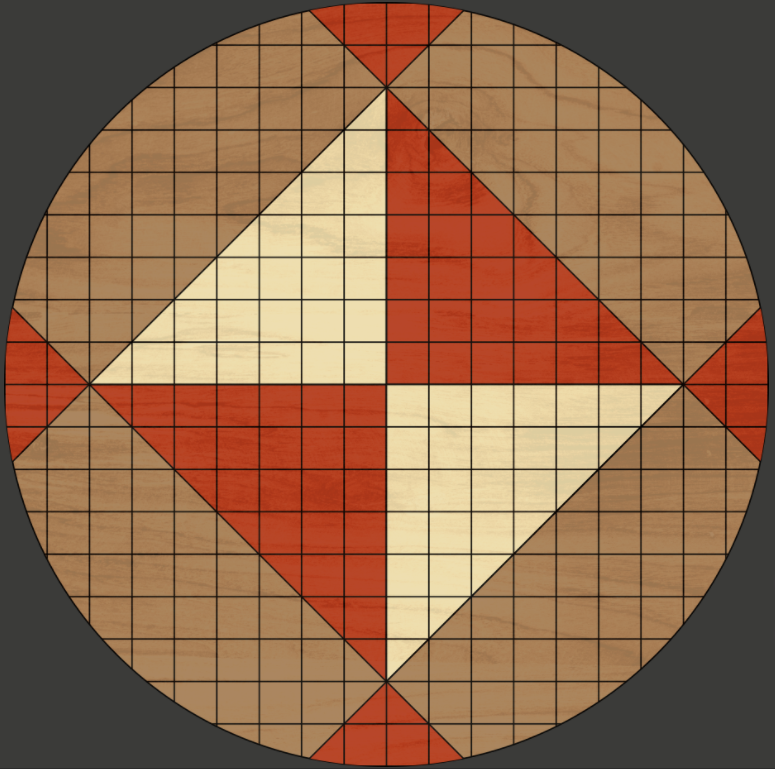
\includegraphics[width=0.6\textwidth]{pictures/board.png}
	\caption{Игровое поле}
	\label{fig:1}
\end{figure}

\section{Особые зоны}

\subsection{Ворота}

Это точки с координатами (8;0), (-8;0), (0;8), (0;-8). Фишки размещаются в любых свободных Воротах, когда помещаются на доску. В ворота можно ставить только цветочные фишки и только в момент размещения их на поле.

\subsection{Сады}
Области разного цвета в центре доски. Базовую цветочную фишку можно переместить только в сад своего цвета. Обратите внимание, что правило распространяется только на точки полностью окруженные садом одного цвета. Например, в центральную точку может попасть любая фишка.

\section{Начало игры}

Перед первым ходом у каждого есть следующий набор фишек:
\begin{itemize}
	\item Четыре Акцентные фишки
	\item Восемнадцать Базовых цветочных фишек — по три Цветочных фишки каждого типа
	\item Две Специальные Цветочные фишки — одна фишка Белого Лотоса, и одна фишка Орхидеи
\end{itemize}

Обычно Хозяин поля играет светлыми фишками, а Гость — темными.

Гость всегда ходит первым. Он выбирает базовую цветочную фишку и помещает ее в ближайшие к себе ворота. Второй игрок будет обязан положить такую же фишку в противоположные ворота. Затем поочередно делаются любые возможны ходы.

\section{Описание ходов}

В свой ход вы либо помещаете новую Базовую цветочную фишку в любые свободные ворота, либо перемещаете свою цветочную фишку по доске. Если вы формируете новую гармонию между своими фишками в ходе перемещения, вы получаете Бонус гармонии, и можете выполнить одно из следующих действий:
\begin{enumerate}[label=\arabic{enumi})]
	\item Поместить акцентную фишку на поле;
	\item Поместить специальную цветочную фишку в ворота;
	\item Если в воротах нет вашей цветочной фишки, поместить туда базовую цветочную фишку;
\end{enumerate}

\section{Специальные цветочные фишки}

У игроков есть по одной Специальной цветочной фишке каждого типа.

\begin{enumerate}
	\item[Орхидея:] перемещается на шесть или менее клеток за один ход. Блокирует соседние цветочные фишки противника. Заблокированные фишки не могут перемещаться сами, но могут гармонировать.
	\item[Белый Лотос:] перемещается на одну или две клетки за один ход. Формирует Гармонии со всеми базовыми цветочными фишками любого игрока. Гармония принадлежит владельцу базовой цветочной фишки. Если у вас есть Белый Лотос на поле, ваша орхидея может быть захвачен любой базовой цветочной фишкой, а также может захватывать цветочные фишки вашего противника.
\end{enumerate}

\section{Акцентные фишки}

У каждого игрока есть по две акцентные фишки каждого типа. Но перед игрой необходимо оставить только четыре любые.

\subsection{Типы Акцентных фишек}

\begin{enumerate}
	\item[Камень:] размещается на свободной точке поля. Отменяет Гармонии на горизонтальной и вертикальной линии, в точке пересечений которых лежит. 
	\item[Колесо:] размещается на свободной точке поля. Перемещает все соседние фишки на одну клетку по часовой стрелке. Если это перемещает фишки с доски, в Ворота, за границы поля, в сад противоположного цвета или перемещает камень, то такой ход считается невозможным.
	\item[Горец:] размещается на свободной точке поля. Отменяет гармонии, созданные с участием соседних фишек.
	\item[Лодка:] размещается на любой Акцентной, Базовой или Специальной цветочной фишке. Может:
	\begin{itemize}
		\item Переместить цветочную фишку на одну клетку в любом направлении(даже по диагонали), занимает место перемещенной фишки.
		\item Удалить любую акцентную фишку с поля.
	\end{itemize}
\end{enumerate}

\section{Завершение игры}

Игра заканчивается:
\begin{itemize}
	\item Либо в тот момент, когда один из игроков формирует круг гармонии.
	\item Либо, когда один из игроков разыгрывает свою последнюю базовую цветочную фишку. В этом случае побеждает игрок с наибольшим числом гармоний, пересекающих центральные линии поля.
\end{itemize}

\chapter{Дебюты}

Дебют определяет ход партии, это очень важная часть почти любой игры. Но вместе с тем в самом начале партии ИИ не могут досчитать до критичных изменений в позиции, а следовательно неверно оценивают позицию и делают глупые(как правило «жадные») ходы. Эта проблема решается дебютной базой. Дебюты в Skud Pai-Sho, в отличии, например, от шахмат принято рассматривать не как последовательность разумных ходов соперников, а как твою стартовую расстановку фишек. На данный момент существует 4 дебюта, которые не дают сопернику серьезного преимущества, рассмотрим их далее.

\section{3-4}

\subsection{Классический 3-4}

Классический дебют 3-4 - это когда вы начинаете с фишки (с дальностью хода)3 и следующим ходом ставите фишку 4 того же цвета в других воротах, или наоборот.
Большинство опытных игроков рекомендуют не использовать дебют 3-4, из-за ограниченной подвижности фишек по сравнению с дебютами 3-5 или 4-5.

\begin{itemize}
	\item Мобильность ваших фишек в начале игры очень низкая.
	\item Вы позднее соберете первую гармонию по сравнению с другими дебютами.
	\item Вы не сможете быстро собрать гармонию в садах, рядом с воротами из которых вы начали игру.
\end{itemize}

\subsection{Альтернативный 3-4}

Альтернативный дебют 3-4 - использовать фишки разного цвета, то есть R3 и W4. Это работает, потому что вы сможете поместить W5 «между» двумя стартовыми фишками. Этот стиль игры сочетает в себе дебюты 3-5 и 4-5.

\begin{itemize}
	\item Больше ваших фишек может войти в сады для создания гармонии, это защищает их от захвата другими базовыми цветами.
	\item Ваши фишки на поле будут разнообразнее.
	\item Вы позднее соберете первую гармонию по сравнению с другими дебютами.
\end{itemize}

\section{3-5}

Дебют 3-5 - это когда вы начинаете с фишки 3 и следующим ходом ставите фишку 5 в других воротах, или наоборот. У этого дебюта есть много возможностей. Хотя у вас может возникнуть соблазн немедленно создать гармонию, подобную А, многие игроки рекомендуют более медленный подход: создание гармонии за 3 или даже 4 следующих хода.

\begin{figure}[!ht]
	\centering
	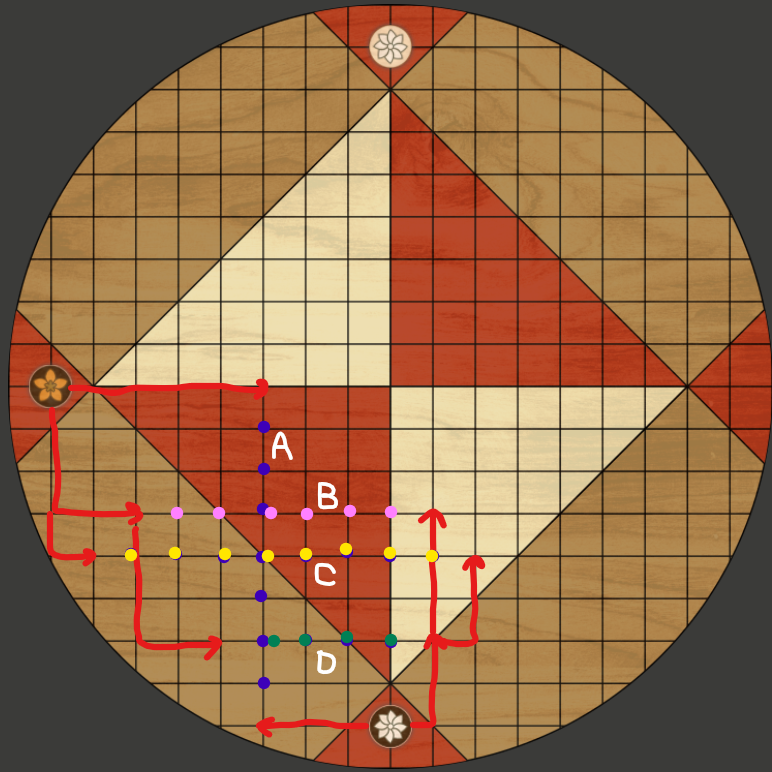
\includegraphics[width=0.6\textwidth]{pictures/3-5.png}
	\caption{Линии гармонии для 3-5}
	\label{fig:2}
\end{figure}

Одним из основных преимуществ дебюта 3-5 является то, что он позволяет игроку размещать свое кольцо гармонии полностью внутри садов, где фишки не могут быть захвачены вражескими базовыми цветочными фишками.

\begin{itemize}
	\item Можно размещать фишки в садах.
	\item Можно создать гармонию всего за 2 хода, если это необходимо.
	\item Мобильность ваших фишек в начале игры низкая по сравнению с дебютом 4-5.
	\item Изолированные фишки, более уязвимы для атак орхидеи соперника.
\end{itemize}

\section{4-5}

Дебют 4-5 - это когда вы начинаете с фишки 4 и следующим ходом ставите фишку 5 того же цвета в других воротах, или наоборот...

\begin{itemize}
	\item Высокая мобильность поставленных фишек.
	\item Фишки не могут попасть в сады противоположного цвета.
\end{itemize}

\section{Итог}

Сильнейшими дебютами считаются 3-5 и 4-5, их вариациями дебютная база ИИ и ограничится. Это возможно, ведь даже если ты хозяин(ходишь вторым) не зависимо от первого ходы ты сможешь использовать по крайней мере одну из этих расстановок.

Здесь стоит отметить, что выбор акцентных фишек тоже должен зависеть от выбора дебюта, однако современная теория не дает ответа на вопрос какие именно фишки с какими дебютами стоит выбирать, это будет выяснено опытным путем — статистикой игр между ИИ с разными дебютными предпочтениями. На этом же этапе будет проверена существующая дебютная теория.

\chapter{Оценочная функция}

Пожалуй самая сложная и важная часть работы. 

Важная, ведь все расчеты так или иначе будут заканчиваться применением к получившейся в конце варианта позиции нашей оценочной функции. И даже если благодаря выбору правильного алгоритма мы сможем получить хорошую глубину и не потерять при этом переспективные варианты , мы все равно будем делать плохие ходы, если неправильно оценим возникающие позиции. 

Сложная, ведь в первую очередь нам важно, не сколько каких фишек расположены на поле, а как они взаимодействуют друг с другом. То есть у нас нет материального ориентира, как, например в шахматах — стоимость расположенных на доске фигур, здесь придется опираться только на динамические факторы.

\section{Оценочная функция}

В качестве первой идеи можно использовать колчество возможных ходов(без учета бонуса гармонии), однако те ходы, которые приводят к созданию гармонии учитывать с коэффициентом 5 + все одиночные гармонии проходящие через центральные линии с коэффициентом 100 + все двойные гармонии, проходящие через обе центральные линии с клэффициентом 1000 + количество акцентных фишек в руке с коэффициентом 1000. Если же на доске победа, то $10^9$ – количество ходов от изначальной до получившейся позиции(чтобы ИИ искал быстрейший способ победить)

Тогда формула оценки позиции:
\begin{equation}
	f(x) = \begin{cases}
		10^9 - steps, & \text{если хозяин выиграл}\\
		-10^9 + steps, & \text{если хозяин проиграл}\\
		g(H) - g(G), & \text{иначе.}
	\end{cases}
\end{equation}

\begin{equation}
	g(x) =  m_{x} + 4 * mh_{x} + 100 * h_{x} + 1000*h2_{x} + 1000*t_{x}
\end{equation}

$m_{G}$, $mh_{G}$, $h_{G}$, $h2_{G}$, $t_{G}$ – мобильность фишек, количество ходов создающих гармонию, количество гармоний, количество двойных гармоний, количество акцентных фишек в руке гостя соответственно, а ($m_{H}$, $mh_{H}$, $h_{H}$, $h2_{H}$, $t_{H}$) – аналогичные измерения для хозяина.

А $steps$ – количество ходов от переданной компьютеру позиции до текущей.

У этой формулы есть несколько способов улучшения:
\begin{enumerate}[label=\arabic{enumi})]
	\item На ранних стадиях игры гораздо важнее сбор кольца, поэтому она высоко оценивает двойные гармонии. Однако, когда на руках у соперников осталось мало базовых цветочных фишек двойная гармония, очевидно, стоит меньше, т.к. при подсчете очков, после выставления на поле последней базовой фишки. Двойная гармония засчитывается как просто 2 гармонии(а не 10 как в формуле). Просто линейно уменьшать стоимость от 10 до 2 в зависимости от колиество оставшихся на руках базовых фишек вряд ли хорошая идея. Нужно собрать статистику.
	\item Что считать двойной гармонией. Исходя из названия, конечно, предпологается что речь о 2х гармониях образованных 3мя фишками и пересекающих обе центральные линии. Но так ли это разумно? Возможно стоит считать двойной гармонией все такие последовательности гармоний, которые можно соединить в кольцо гармонии, добавив одну фишку. Тогда стоит менять стоимость такой двойной гармонии в зависимости от того как быстро и сколькими способами это можно сделать. Стоит ли учитывать препятствия на пути таких цепочек? Если да, то как? Для ответов необходимо собрать статистику.
	\item Формула только косвенно учитывает специальные цветочные фишки. Это не так критично как может показаться на первый взгляд. Эти фишки не слишком сильны. Ведь лотос медленный, а орхидея в начале игры тратит слишком много времени на перемещения, так как ни с кем не гармонирует и ее перемещение не дает никаких бонусов, а в середине игры, когда фишек и потерянное время не так критично на доске стоит уже много фишек и съедение одной из низ них почти всегда будет означать и съедение орхидеи. Так что они могут быть автоматически учтены просто за счет глубины поиска по дереву игры. Но это может оказаться самообманом. 
	\item При подсчете стоимости mh стоит учитывать, что множества способов собрать одну и ту же гармонию могут стоить по разному не только в зависимости от количество этих способов. Например, 2 фишки R4 и R5, расположенные на одну клетку по диагонали друг от друга в центре доски дадут нам 24 варианта собрать гармонию, однако все они почти ничем не будут отличаться друг от друга, а те же R4 и R5 расположенные на клетках (1; 7) и (4; -7) дадут всего 2 варианта собрать из них гармонию за один ход, однако такие 2 построения будут сильно друг от друга отличаться и сбор гармонии таких фишек сложнее блокировать акцентными фишками, чем 24 варианта из первого примера. Вероятно стоит уменьшать коэффициент mh собираемый одними и теми же фишками, а так же отдельно с разными коэффициентами считать сбор гармонии пересекающий центральную линию и нет.
\end{enumerate}

\section{Машинное обучение}
Так же есть принципиально другой подход к получению оценочной функции — машинное обучение. Однако его использование возможно будет только в конце работы, как возможное усиление ИИ. Сейчас это невозможно из-за банального отсутствия базы партий в Skud Pai-Sho, а тем более качественных партий, так что обучать просто не на чем, однако я буду сталкивать между собой созданные мной варианты ИИ и под конец это может стать действительно хорошим решением.

\section{Вывод}
Существует много различных способов оценить позицию, нужно будет реализовывать их и сталкивать за игрой различные варианты оценки на разных алгоритмах. Не стоит забывать о том, что доска в Pai-Sho достаточно большая(249 мест для фишки), вариантов хода каждой фишки много и перечисленные характеристики посчитать не просто, возможно придется где-то жертвовать точностью оценки ради возможности посчитать дальше в глубину и искать более простые характеристики для формулы.

\chapter{Алгоритмы}

Очевидной проблемой при выборе алгоритма для Skud Pai-Sho является огромное количество вариантов хода в середине игры. Даже в приведенном в предыдущей главе примере с двумя фишками R4 и R5 в середине доски, если у игрока есть на руках одновременно камень, горец и колесо, то только ходы со сбором гармонии между двумя этими фишками дадут чуть меньше чем 24*(249+1)*3 = 18000 вариантов хода. Для сравнения в шахматах, всего вариантов хода в среднем 50-60. Говоря о таких огромных числах, очевидно, что полный перебор едва ли сможет просчитать и на 2 полухода. Но, проблема, конечно, не только в этом, даже быстрый алгоритм Монте Карло будет тратить очень много времени на прогон 1000 симуляций на каждый ход, даже если речь пойдет хотя бы о 100000 вариантов хода(их все нужно банально найти перед тем как выбрать случайный, а это в лучшем случае O(количества ходов)). Скорее всего большинство ходов надо будет отбрасывать даже не проверяя. Сложно заранее оценить сколько ходов будет после отбрасывания «бессмысленных», но я предлогаю ориентироваться на 100-500. Тогда хоть какие-то алгоритмы становятся возможными и даже полный перебор уже даст по крайней мере 4 полухода.

\section{Коэффициент ветвления}

Подробнее остановимся на коэффициенте ветвления. Попробуем оценить сверху и найти среднее значение для имеющихся в нашем распоряжении турнирных партий.

Если на доске все 20 цветочных фишек и все их ходы возможны, то мы получим 6*24 + 6 * 38 + 6 * 52 + 12 + 70 = 766. Если каждый из этих ходов собирает гармонию(орхидея может уйти с пути гармонии) и у нас на руках все 4 вида акцентных фишек, то мы получим 766 * 249 + 766 * (7 + 18*2*8) = 416704.

Рассмотрим среднее значение в реальных партиях, чтобы получить действительно осмысленные партии возьмем финал ... Будем рассматривать ходы начиная с 4го, так как первые три хода почти формальные, к тому же определяются дебютной теорией и не интересны для нашей задачи.(TODO)

\section{Бессмысленные ходы}

Отбрасывание бессмысленных вариантов будет общей идеей, не относящейся к конкретному алгоритму, поэтому обсудим ее отдельно.

Основная масса вариантов появляется при выборе места для акцентной фишки, так что рассмотрим в начале их. Во-первых, акцентных фишек дается всего 4 на игру и они очень ценные, поэтому редко вообще стоит их трогать, но это больше относится к оценочной функции. Во-вторых, некоторые акцентные фишки действительно становятся бесполезными в различных позициях.

Так камень нет смысла ставить на точки, которые расположены на пересечении горизонтали и вертикали, на которых нет ни одной базовой цветочной фишки соперника. 
Аналогично для колеса, причем выставление колеса в точку, вокруг которой нет ни одной фишки крайне подозрительно, скорее всего, даже несмотря на то, что можно придумать позицию, в которой это будет хорошим ходом. Такие ходы стоит сразу отметать, как почти наверняка бессмысленные. 

Остался горец, с ним сложнее, точно бесполезными будут ходы в места, где на горизонтали и вертикали фишки, а так же на соседних горизонтали и вертикали нет ни одной вражеской фишки, что скорее всего почти не изменит количество вариантов хода.
 
Скорее всего для защитных фишек(камень и горец) вообще придется расписывать, что их надо ставить, только в места, куда не хватает одной фишки до кольца гармонии или в конце партии в большие скопления гармонирующих фишек.

\section{Полный перебор и Альфа-Бета отсечение}

В основе этих алгоритмов лежит стандартный минимакс, они отличаются только тем как выбирается набор ходов для рассмотрения на каждом шаге.

Как и следует из названия «Полный перебор», здесь мы просто переберем все варианты, в надежде на глубину 2-4 полухода(в зависимости от того будем мы предварительно отсекать бессмысленные ходы или нет). Особых надежд на то, что это может дать хороший результат нет, но это важно реализовать для сравнения. Если какой-то алгоритм проигрывает полному перебору, то мы отсекаем какие-то хорошие продолжения, а значит функции выбора надо менять.

Альфа-бета отсечение нельзя назвать оптимизацией полного перебора, хотя на первый взгляд так может показаться. Идея алгоритма в том, чтобы отсекать не перспективные относительно других варианты. Это значительно ускоряет полный перебор(или дает возможность спуститься дальше по дереву игры). Однако это не оптимизация, так как на первый взгляд не перспективные ходы могут оказаться  лучшими при углублении в позицию(результат меняется).

\section{Монте Карло}

В чистом виде этот алгоритм предпологает, что мы запускаем несколько симуляций до завершения партии(здесь симуляция — это игра из заданной позиции в которой оба соперника делают случайные ходы), смотрим, для какого хода симуляции набирают больше очков и его считаем лучшим.

Популярным его улучшением является выбор внутри каждой симуляции с большей вероятности того хода, который набрал больше очков в предыдущих симуляциях. Основным преимуществом такого подхода будет то, что сложность анализа не так сильно увеличивается от количества вариантов хода.

Две, основных, на мой взгляд, проблемы очень похожи. Во-первых, в средней позиции, ходов, завершающих игру сбором кольца гармонии будет почти 0, и впринципе их может быть 1-2, ходов, которые уменьшают количество базовых цветочных фишек на руке максимум 6*4=24, а вот просто перемещающих фишки ходов базовые цветочные фишки дают 24, 38 или 58 соответственно, почти каждый из этих ходов, как правило, возможен и количество цветков на поле будет постоянно увеличиваться, пока у одной из сторон их не станет 18(примерно, от 38+58=96 до 17*38=646(число не точное, т.к. зависит от того, какой цветок поставим последним и как они расположены), взятия крайне моловероятны), т.е. большинство ходов никак не приближают конец игры, что может дать нам почти бесконечную игру. В расчетах выше я не учитывал варианты дополнительных движений за счет бонуса гармонии, их имеет смысл учитывать не как продолжение хода, а как слкдующий ход, который становится возможен, если была собрана гармония, эти две проблемы значительно усложняются.

Я думаю, что хорошим решением будет использовать гибрид — то есть досчитывать до какой-то глубины симуляцию, а к результату применять оценочную функцию. Так мы и ускорим симуляции, и учтем возможность победы с помощью кольца гармонии. Причем как я уже писал, чем ближе к концу игры тем больше влияние альтернативного условия победы, а следовательно тем эффективнее оценивают позицию, так что глубину симуляции можно не задавать константно, а менять в зависимости от текущей позиции(не слишком глубоким анализом, например, в зависимости от количества базовых цветочных фишек на руках). К тому же, можно заметить, что просто применение оценочной функции, это просчет с помощью альфа-бета отсечения с глубиной 0, тогда видно, что 0 — это совсем не обязательный параметр и после симуляции мы можем делать просчет на заданную глубину. При этом поскольку, мы будем собирать статистику, а не пытаемся просчитывать точные варианты, оценочная функция может быть не такой точной, а просто в большинстве позиций уметь правильно понять кто побеждает.

\chapternonum{Заключение}

Написание ИИ для Skup Pai-Sho действительно сложная задача, по многим причинам — относительно сложное описание множества возможных ходов, большое количество вариантов хода, строго динамические характеристики позиции и т.д. Однако все эти проблемы не являются неприодолимыми препятствиями, подробно описанные выше методы, такие как дробление одного хода на составляющие, запрет бессмысленных ходов, отсечение ходов с низкой промежуточной оценкой, симуляции, дебютная база, машинное оучение для оценки позиции вполне могут справится с поставленной задачей. Остается только реализовать описанные варианты и проверить их эффективность в бою.

\renewcommand{\bibname}{Список литературы} 

\begin{thebibliography}{4}

\bibitem{TeX:YarSU}
	SKUD PAI SHO COMPREHENSIVE RULES [Электронный ресурс].URL: \url{https://skudpaisho.com/site/games/skud-pai-sho/pai-sho-rules/}
	(дата доступа: 07.02.2021).

\bibitem{TeX:YarSU}
	Skud Pai Sho: Unofficial Strategy Guide [Электронный ресурс]. URL:\url{https://docs.google.com/document/d/1q-eMxZiJEiT347lWbhJ3ojS5-J6sB2yaulih9YEdhMo}
	(дата доступа: 07.02.2021).

\bibitem{TeX:YarSU}
	Скуд Пай-Шо [Электронный ресурс]. URL:\url{https://docs.google.com/document/d/1XKUwkTFUMi5RPrR_dIV6mVAVlPO3zCJvBtiUMKamGLY}
	(дата доступа: 07.02.2021).

\bibitem{TeX:YarSU}
	Skud Pai Sho: Перевод неофициального гайда по стратегиям [Электронный ресурс]. URL:\url{https://docs.google.com/document/d/1ogBxcEn2lv5ZAMt9I1P0F1z3wXA_5w3wg58j2iNcuFg}
	(дата доступа: 07.02.2021).

\end{thebibliography}

\end{document}
